\documentclass[../main.tex]{subfiles}

\begin{document}
	
En el presente capítulo comenzaremos con la definición de una categoría libre junto a los lenguajes que producen. Posteriormente, probaremos que son equivalentes a los lenguajes regulares, aquellos producidos por un autómata finito, y finalizaremos mostrando la implementación en \py{Python}.
\section{Categorías libres}
\nota{¿incluir la definición de categoría?}
\begin{dfn}
	Una \textbf{signatura simple} \(G\) (o gráfica dirigida) es una conjunto de vértices \(G_0\) y uno de aristas \(G_1\) tal que cada arista tiene asociado dos vértices, un dominio y un codominio
	$$\signature{G_1}{G_0}$$
	Dadas \( G, \Gamma\) signaturas simples, un \textbf{homomorfismo de signaturas} \( \phi:G \to \Gamma\) es un par de funciones \( \phi_0: G_0 \to \Gamma_0\) y \( \phi_1: G_1 \to \Gamma_1\) tal que el siguiente diagrama conmuta: 
	\[
	\begin{tikzcd}
		G_0 \arrow{d}{\phi_0} & G_1 \arrow{r}{\tt{dom}} \arrow{l}{\tt{cod}} \arrow{d}{\phi_1} & G_1 \arrow{d}{\phi_0} \\
		\Gamma_0 & \Gamma_1 \arrow{r}{\tt{dom}} \arrow{l}{\tt{cod}} & \Gamma_1
	\end{tikzcd}
	\]
\end{dfn}

Observemos que si consideramos dos homomorfismos de signaturas $\phi=(\phi_0, \phi 1): G \to \Gamma$ y $\psi =(\psi _0, \psi_1): \Gamma \to \Phi$ 
podemos tomar su composición entrada a entrada, es decir, $\psi \circ \phi = (\psi_0 \circ \phi_0,\psi_1 \circ \phi_1)$, la  cual resulta nuevamente un homomorfismo de signaturas, pues el siguiente diagrama

\[
\begin{tikzcd}
	G_0 \arrow{d}{\phi_0} & G_1 \arrow{r}{\tt{dom}} \arrow{l}{\tt{cod}} \arrow{d}{\phi_1} & G_1 \arrow{d}{\phi_0} \\
	\Gamma_0 \arrow{d}{\psi_0} & \Gamma_1 \arrow{r}{\tt{dom}} \arrow{l}{\tt{cod}} \arrow{d}{\psi_1} & \Gamma_1 \arrow{d}{\psi_0} \\
	\Phi_0 & \Phi_1 \arrow{r}{\tt{dom}} \arrow{l}{\tt{cod}} & \Phi_1 \\
\end{tikzcd} 
\]

conmuta ya que el superior y el inferior lo hacen. \\
Notemos, además, que la composición anterior es asociativa, pues lo es en cada entrada y que la identidad $Id_\Gamma=(Id_{\Gamma_0}, Id_{\Gamma_1})$ 
satisface que $Id_\Gamma \circ \phi = \phi$ y $\psi \circ Id_\Gamma = \psi$. Por lo tanto, tenemos una categoría cuyos objetos son las signaturas simples y sus flechas son los homomorfismos, la cual denotaremos $\bf{Graph}$. \\

Por otro lado, podemos considerar la categoría \( \bf{Cat} \) cuyos objetos son categorías y las flechas son funtores entre ellas. Con esto, definimos el siguiente funtor:
\[
	\bf{U} : \bf{Cat} \to \bf{Graph}
\]
tal que para cada categoría $\mathcal{C}$, $\bf{U}\mathcal{C}$ es la gráfica dirigida cuyos vértices son los objetos, $Ob(\mathcal{C})$, y los aristas corresponden a los morfismos, $Mor(\mathcal{C})$. Además, notemos que cada funtor $f: \cal{C} \to \cal{C'}$ induce a un homomorfismo de gráficas $\bf{U} f: \bf{U}(\cal{C}) \to \bf{U}(\cal{C'})$. \\
Puesto que el funtor $\bf{U}$ lo único que hace es olvidar la composición de morfismos en una categoría para obtener la gráfica asociada, decimos que es un funtor olvidadizo. \\
Ahora, nuestro objetivo es definir un funtor $$\bf{F}: \bf{Graph} \to \bf{Cat}$$. \\
Dada una gráfica dirigida $G$, los objetos de $\bf{F}G$ serán los vértices de $G$, y sus morfismos serán de las siguientes dos formas:
\begin{itemize}
	\item Para cada $v$ vértice de $G$, tenemos un morfismo $Id_v: v \to v$; y
	\item para cualquier $n \in \mathbb{N}$ y para cualesquiera $e_1, ... , e_n$ aristas de $G$ tales que $\tt{cod} (e_i)=\tt{dom} (e_{i+1})$ con $i \in \{ 1, ..., n-1\}$ tenemos un morfismo $e_1 \dots e_n : \tt{dom} (e_1) \to \tt{cod} (e_n)$.
\end{itemize}
Es decir, los morfismos corresponden a las identidades y a todos los posibles caminos dentro de la gráfica. La composición de dos caminos está dada por la concatenación, mientras que componer con la identidad actúa de la manera esperada. \\ 
Como la concatenación es siempre asociativa, claramente tenemos que $\bf{F}(G)$ es una categoría. \\
Ahora, tomemos $\phi: G \to G'$ un homomorfismo de gráficas, definimos el funtor $\bf{F}\phi: \bf{F}(G) \to \bf{F}(G')$ de la siguiente manera:   
\begin{itemize}
	\item Para cada $v$ objeto en $\mathbf{F} (G)$, $(\mathbf{F}\phi)(v)=\phi_0(v) $;
	\item Para cada $I_v$ morfismo identidad de $\mathbf{F} (G)$, $(\mathbf{F}\phi)(I_v)=I_{\phi_0(v)} $; y 
	\item Para cada $E:e_1 \dots e_n$ morfismo camino de $\mathbf{F} (G)$, $(\mathbf{F}\phi)(e_1 \dots e_n)=\phi(e_1) \dots \phi(e_n)$
\end{itemize}
Hagamos notar que el último inciso está bien definido pues $\phi$ es un homomorfismo de gráficas. \\
Con lo anterior, estamos en condiciones de probar nuestra primera proposición: 

\begin{prop}
	Sea $G$ una gráfica dirigida. Entonces existe un morfismo de gráficas $\eta:G \to \mathbf{UF}G$ tal que para cualquier categoría $\cal{C}$ y un homomorfismo de gráficas $\phi: G \to \mathbf{U}\cal{C}$ existe un único funtor $\phi': \mathbf{F}G \to \cal{C}$
	que hace conmutar el siguiente diagrama:
	
	\[
	\begin{tikzcd}
		G \arrow{r}{\eta} \arrow{rd}{\phi} & \mathbf{UF}G \arrow{d}{\mathbf{U}\phi'} \\
		& \mathbf{U}\cal{C}
	\end{tikzcd}
	\] 	
\end{prop}
\begin{proof}
	Definimos $\eta:G \to \mathbf{UF}G$ como $\eta_1$ la identidad en vértices y dado un arista $e:v_1 \to v_2$ en $G$, entonces $\bar{e}$ es un morfismo en $\mathbf{F}G$, y así $\eta(e)=e:v_1 \to v_2$ un arista en $\mathbf{UF}G$. Claramente es un morfismo de gráficas.   
	\nota{Pendiente.}
\end{proof}
Observemos que el teorema nos indica que dada una gráfica $G$, el funtor $\mathbf{F}$ construye la categoría libre generada por $G$, la cual denotaremos como $\mathbf{C}(G)$
\begin{prop}
	El funtor libre $\mathbf{F: Graph \to Cat}$ es adjunto izquierdo del funtor olvidadizo $\mathbf{U: Cat \to Graph}$
\end{prop}

\begin{proof}
	\nota{Pendiente}
\end{proof}

\newpage

\section{Lenguaje en una categoría libre}
Nuestro objetivo ahora será definir el lenguaje generado por una signatura simple (o gráfica dirigia) y posteriormente mostrar que son exactamente los lenguajes regulares. \\
Sea $V$ un vocabulario (o léxico) no vacío y $G$ una signatura simple. A cada arista de $G$ le asociaremos una palabra en $V$, mediante una función $L: G_0 \to V$, o equivalentemente, un homomorfismo de gráficas $L: G \to V$ donde $V$ es la gráfica con un vértice y cada palabra es un arista. Observemos que podemos extender $L$ de la siguiente forma: para cada morfismo $f=f_n \circ \dots \circ f_1$ en \textbf{C}$(G)$, $L^*(f)=L(f_1)\cdots L(f_n) \in V^*$ y $L^*(Id_v)=\varepsilon$ para cualquier $v \in G_0$. 

\begin{dfn}
	Una \textbf{gramática simple} es un signatura finita simple $G$ junto a un homomorfismo de gráficas $L: G \to V$ donde $V$ es un conjunto de palabras, el vocabulario, y símbolos distinguidos $s_0, s_1 \in G_0$, llamados el símbolo inicial y el terminal. Así, tenemos el siguiente diagrama:  
	
	\[
	\begin{tikzcd}
		G_0 & G_1 \arrow{l}{\texttt{dom}} \arrow{r}{\texttt{cod}} \arrow{d}{L} & G_0 \\
		& V &
	\end{tikzcd}
	\]
	
	El lenguaje generado por $G$ se define como: \\
	\[
		\mathcal{L}(G)=L^*(\textbf{C}(s_0,s_1)) \subset V*
	\]
	Un morfismo de gramáticas simples $\phi : G \to H$ es un homomorfismo de gráficas tal que el siguiente diagrama conmuta:
	
	\[
		\begin{tikzcd}
			G \arrow{rr}{\phi} \arrow{rd}{L_G} & & H \arrow{ld}{L_H} \\
			& V &
		\end{tikzcd}
	\]
	
\end{dfn}

\begin{ej}
	Consideremos la siguiente gráfica $G$: 
	\begin{center}
	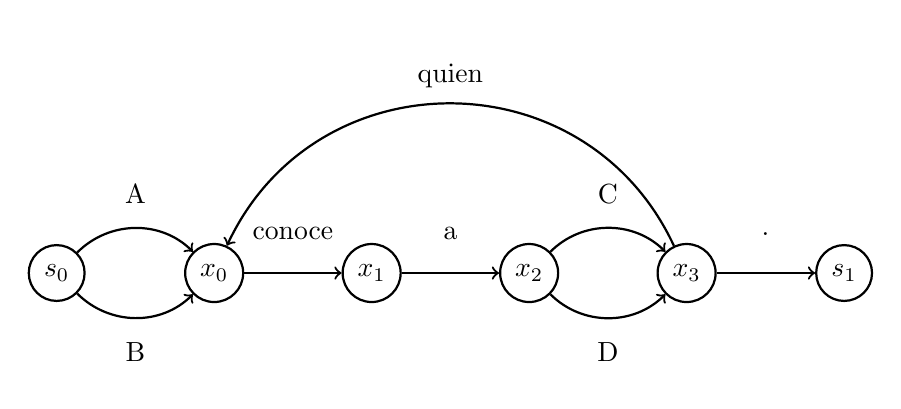
\begin{tikzpicture}[node distance={20mm}, thick, main/.style = {draw, circle},
	protein/.style={circle,draw=white,very thick}] 
		\node[main] (1) {$s_0$}; 
		\node[main] (2) [right of=1] {$x_0$}; 
		\node[main] (3) [right of=2] {$x_1$}; 
		\node[main] (4) [right of=3] {$x_2$}; 
		\node[main] (5) [right of=4] {$x_3$}; 
		\node[main] (6) [right of=5] {$s_1$}; 
		\node[protein] (p) at (1,1)  {A};
		\node[protein] (p) at (1,-1)  {B};
		\node[protein] (p) at (3,.5)  {conoce};
		\node[protein] (p) at (5,.5)  {a};
		\node[protein] (p) at (5,2.5)  {quien};
		\node[protein] (p) at (7,1)  {C};
		\node[protein] (p) at (7,-1)  {D};
		\node[protein] (p) at (9,.5)  {.};
		\draw[->] (2) -- (3);
		\draw[->] (3) -- (4);
		\draw[->] (5) -- (6);
		\draw[->] (1) to [out=45, in=135, looseness=1] (2); 
		\draw[->] (1) to [out=315, in=225, looseness=1] (2); 
		\draw[->] (5) to [out=115, in=65, looseness=1.2] (2);    
		\draw[->] (4) to [out=45, in=135, looseness=1] (5); 
		\draw[->] (4) to [out=315, in=225, looseness=1] (5); 
	\end{tikzpicture}
	\end{center}	
	Observemos que induce una gramática simple, y una oración ''A conoce a C quien conoce a D.'' está en el lenguaje generado por dicha gramática. 
\end{ej}
	

 \begin{dfn}
 	
 	Una gramática regular es una tupla $(N,V,P,s_0)$ donde $V$ es un vocabulario no vacío; $N$ es un conjunto de símbolos no terminales con un símbolo de inicio $s_0$; y $P$ un conjunto finito de reglas de producción, cada una de alguna de las siguientes formas:
 	
 	$$A \to aB$$
 	$$A \to a$$
 	$$A \to \epsilon$$
 	
 	con$A$ y $B$ en $N$, y $a \in V$. \\
 	Una derivación es la aplicación consecutiva de reglas de producción. \\
 	Definimos el lenguaje $L$ generado por una gramática regular como $w\in V*$ está en $L$ si y sólo si existe una derivación de $s_0$ a $w$. \\
 	Decimos que un lenguaje es regular si es generado por un gramática regular.
 \end{dfn}
 
 \begin{ej}
 	Consideremos la siguiente gramática regular con los símbolos no terminales $N= \{A, s_0\}$, el vocabulario $V=\{a, b, c\}$ y con las siguientes reglas $P$:
 	\begin{align*}
		s_0 &\to as_0 \\
		s_0 &\to bA \\
		A &\to \epsilon \\
		A &\to cA
 	\end{align*} 
 	Observemos que el lenguaje generado por dicha gramática es $L=\{ a^i b c^j|i, j \in \mathbb{N} \}$  
 \end{ej}
 
 Con la definición anterior, ya estamos en condiciones para demostrar el teorema principal de este capítulo:
 
 
 \begin{thm}
	\begin{enumerate}[label=(\alph*)]
 		\item Todo lenguaje regular es generado por una gramática simple.
 		\item Todo lenguaje generado por una gramática simple es regular.
 \end{enumerate}	

 \end{thm}
 
 \begin{proof}
 	
 	
 	Primero probemos $(a)$.\\
 	Sea $L$ un lenguaje regular generado por la gramática $(N,V,P,s)$. \\
 	Definimos una gramática simple $G=P \rightrightarrows (V \cup \{ s, \epsilon \})$ donde para cada $p$ regla de producción:
 	\begin{itemize}
 		\item Si $p$ es de la forma $A \to aB$ con $A,B \in N$ y $a \in V$ entonces $p:A \to B$ en $G$ y $L(p)=a$.
 		\item Si $p$ es de la forma $A \to a$ con $A \in N$ y $a \in V$, entonces $p:A \to s_1$ en $G$ y $L(p)=a$
 		\item Si $p$ es de la forma $A \to \epsilon$ con $A \in N$, entonces $p:A \to s_1$ en $G$ y $L(p)=\epsilon$
 	\end{itemize}
 	
 	Observación. El símbolo $\epsilon$ de nuestro vocabulario cubrirá el papel de la cadena vacía. \\
 	
 	Probemos que $L=L(G)$.\\
 	Sea $w \in L$. 
 	Entonces existe una derivación
 	\[ s_0 \xrightarrow{p_1} \cdots \xrightarrow{p_n} w\]
 	Observemos que si $n=1$, entonces $p_1$ es de la forma $s \to w$, así tenemos el morfismo $p_1: s_0 \to s_1$ tal que $L(p_1)=w$.
 	Ahora, si $n>1$ veamos que la derivación es necesariamente de la forma: 
 	\[ s_0 \xrightarrow{p_1} aA_1 \xrightarrow{p_2} \cdots \xrightarrow{p_{n-1}} uA_{n-1} \xrightarrow{p_n} w\]
 	donde $A_i \in N$ con $i \in \{ 1, ..., n-1 \}$, $a\in V$ y $u \in V^*$. Así tenemos los siguientes morfismos en $G$: 
 	
 	\[ s_0 \xrightarrow{p_1} A_1 \xrightarrow{p_2} \cdots \xrightarrow{p_{n-1}} A_{n-1} \xrightarrow{p_n} s_1\]
 	
 	Entonces el morfismo $p =  p_n \circ p_{n-1} \circ \dots \circ p_2 \circ p_1: s_0 \to s_1$ y
 	\begin{align*}
	 	 L(p)=L(p_n \circ p_{n-1} \circ \dots \circ p_2 \circ p_1) &=(L(p_1) L(p_2) \dots L(p_n)) L(p_{n-1}) \\
	 	 &= u L(p_{n-1}) = w
 	\end{align*}
 	Observemos que es posible que $L(p_{n-1}) = \epsilon$ pero en ese caso $u = u \epsilon = w$. \\
 	Por lo tanto, $w \in L(G)$. Así, $L \subset L(G)$\\
 	Ahora, sea $w \in L(G)$. 
 	Entonces existe $f:s_0 \to s_1$ en \textbf{C}$(G)$ tal que $L(f)=w$. Como \textbf{C}$(G)$ es una categoría libre, entonces $f$ es un camino en $G$, así existen $p_1, \dots, p_n$ reglas de producción en $P$ tal que $f=p_n \circ ... \circ p_1$ que inducen un derivación: 
 	\[
 		s_0 \xrightarrow{p_1} \cdots \xrightarrow{p_n} w
 	\]
 	Y, por lo tanto, $w \in L$. Así $L(G) \subset L$. \\
 	Con ello concluimos que $L=L(G)$ y terminamos la prueba del inciso (a). \\
 	Vayamos con la prueba de (b) \\
 	Sea $G$ una gramática simple con el homomorfismo $L: G \to V$ con $V$ vocabulario. \\
 	La estrategia será construir un autómata finito no determinista que admite el lenguaje $L(G)$, lo cual implica que $L(G)$ es un lenguaje regular. \\ \nota{Agregar referencia} \\
 	Definimos el AFND $M$ de la siguiente manera: su conjunto de estados es $G_1$, es decir, los vértices de $G$, donde $s_0$ es el símbolo de inicio y $F=\{s_1\}$ el conjunto de estados finales, y tomemos $V$ como el conjunto de entradas. Definimos la función de transición $\delta : G_0 \times V \to 2^{G_0}$ tal que para cada $q \in G_0$ y $v\in V$, 
 	\[
 		\delta (q,v) = \{q'|\exists f: q \to q' \in G_1 \text{ tal que }L(f)=v \}
 	\]
 	Recordemos que $\delta$ se extiende recursivamente a $V*$ de la siguiente manera:
 	\begin{align*}
 		&\delta ^* (q, \epsilon) = \{ q \} \\
 		&\delta ^* (q, xa) = \bigcup_{r \in \delta ^* (q,a)} \delta (r,a)
 	\end{align*}
	Así, definimos el lenguaje aceptado por $M$ como:
	\[
		L(M)=\{x \in V^* | \delta ^* (s_0, x) \cap {s_1} \neq \varnothing \}
	\]
 	Probemos que $L(G)=L(M)$. \\
 	Sea $w \in L(G)$. Entonces existe $f:s_0 \to s_1$ en $\mathbf{C}(G)$ tal que $L(f)=q$. Observemos que entonces existen $f_1, \dots, f_n$ en $G_1$ tales que el siguiente diagrama conmuta: 
 	\begin{center}
 	\begin{tikzcd}
 		a_0=s_0 \arrow{r}{f_1} \arrow[rrrr,bend right, swap]{f} & a_ 1 \arrow{r}{f_2} & ... \arrow{r}{f_{n-1}} & a_{n-1} \arrow{r}{f_n} & s_1=a_{n+1}
 	\end{tikzcd}
	\end{center}
 	Así $q=L(f)=L(f_1) \cdots L(f_n)$, entonces observemos que para cada $i\in \{0, ..., n\}$, $a_{i+1} \in \delta (a_i, L(f_i))$ y, por lo tanto, $s_1=a_{n+1} \in \delta ^*  (a_0, L(f))=\delta ^*  (s_1, w)$. Como $\{s_1\}$ es el conjunto terminal, concluimos que $w \in L(M)$.  Por lo tanto, $L(G) \subset L(M)$. \\
 	Sea $w \in L(M)$ \\
 	Entonces $s_1 \in \delta ^* (s_0, w)$. \\
 	Observemos que si $w= \epsilon$, entonces $s_1 \in \delta (s_0, \epsilon)$, así hay un morfismo $f:s_0 \to s_1$ tal que $L^*(f)= \epsilon$, por la definición de $L^*$ esto implica que $f=Id_{s_0}$, así $s_0=s_1$ y $w \in L(G)$. \\ 
 	Por otro lado, si $w$ no es la cadena vacía, entonces hay $w_1,\dots, w_n \in V$ tales que $w=w_1 \cdots w_n$ y estados $q_1, \dots, q_{n-1}$ que satisfacen:
 	\begin{multicols}{3}
 		$q_1 \in \delta (s_0,w_1)$ \\
 		$q_{i+1} \in \delta (q_i,w_i)$ \\
 		$s_0 \in \delta (q_{n-1},w_n)$
 	\end{multicols} 
 	para $i \in \{ 1, ..., n-2 \}$. Esto significa que hay $f_1, \dots , f_n$ en $G_1$ tales que
 	
 	 \begin{center}
 		\begin{tikzcd}
 			s_0 \arrow{r}{f_1}  & q_ 1 \arrow{r}{f_2} & ... \arrow{r}{f_{n-1}} & q_{n-1} \arrow{r}{f_n} & s_1
 		\end{tikzcd}
 	\end{center}
 	y $L(f_i)=w_i$ con $i \in \{1, \dots n\}$. Por lo tanto, $f_n \circ ... \circ f_1 : s_0 \to s_1 \in \mathbf{C}(G)$ y 
 	\[
 		L^*(f_n \circ ... \circ f_1) = L(f_1) \cdots L(f_n)=w_1 \cdots w_n = w
 	\]
 	Por lo tanto, $w \in L(G)$ y así $L(M) \subset L(G)$. \\
 	Por ello, $L(G)=L(M)$ como queríamos demostrar. 
 \end{proof}
 
 A partir de ahora dejaremos de usar el término gramáticas simples y, en virtud del teorema anterior, las llamaremos gramáticas regulares. Denotaremos como $\mathbf{Reg_V}$ a la categoría cuyos objetos son gramáticas regulares y los morfismos son los homomorfismos entre ellas. 
 
 Para ilustrar las pruebas anteriores, veamos los siguientes ejemplos:
 
 \begin{ej}
 	Consideremos la gramática regular del segundo ejemplo, observemos que su lenguaje es generado por la gramática de la siguiente gráfica:
 	
	\begin{center}
	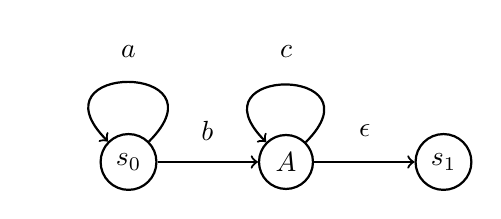
\begin{tikzpicture}[node distance={20mm}, thick, main/.style = {draw, circle},
		protein/.style={circle,draw=white,very thick}] 
		\node[main] (1) {$s_0$}; 
		\node[main] (2) [right of=1] {$A$}; 
		\node[main] (3) [right of=2] {$s_1$};
		\draw[->] (1) -- (2);
		\draw[->] (2) -- (3); 
		\draw[->] (1) to [out=45, in=135, looseness=7] (1);
		\draw[->] (2) to [out=45, in=135, looseness=7] (2);
		\node[protein] (p) at (0,1.4)  {$a$};
		\node[protein] (p) at (2,1.4)  {$c$};
		\node[protein] (p) at (1,.4)  {$b$};
		\node[protein] (p) at (3,.4)  {$\epsilon$};
	\end{tikzpicture}
	\end{center}
	Vale la pena notar que esta gráfica induce inmediatamente un autómata finito con épsilon transiciones. 
 \end{ej}
 	
 \begin{ej}
	 Consideremos la gramática regular del primer ejemplo, es claro que induce el siguiente AFND:
	 \begin{center}
	 	\begin{tikzpicture}[node distance={20mm}, thick, main/.style = {draw, circle},
	 		protein/.style={circle,draw=white,very thick}] 
	 		\node[main] (1) {$s_0$}; 
	 		\node[main] (2) [right of=1] {$x_0$}; 
	 		\node[main] (3) [right of=2] {$x_1$}; 
	 		\node[main] (4) [right of=3] {$x_2$}; 
	 		\node[main] (5) [right of=4] {$x_3$}; 
	 		\node[state, accepting] (6) [right of=5] {$s_1$}; 
	 		\node[protein] (7) [left of=1] {$start$};
	 		\node[protein] (p) at (1,1)  {A};
	 		\node[protein] (p) at (1,-1)  {B};
	 		\node[protein] (p) at (3,.5)  {conoce};
	 		\node[protein] (p) at (5,.5)  {a};
	 		\node[protein] (p) at (5,2.5)  {quien};
	 		\node[protein] (p) at (7,1)  {C};
	 		\node[protein] (p) at (7,-1)  {D};
	 		\node[protein] (p) at (9,.5)  {.};
	 		\draw[->] (7) -- (1);
	 		\draw[->] (2) -- (3);
	 		\draw[->] (3) -- (4);
	 		\draw[->] (5) -- (6);
	 		\draw[->] (1) to [out=45, in=135, looseness=1] (2); 
	 		\draw[->] (1) to [out=315, in=225, looseness=1] (2); 
	 		\draw[->] (5) to [out=115, in=65, looseness=1.2] (2);    
	 		\draw[->] (4) to [out=45, in=135, looseness=1] (5); 
	 		\draw[->] (4) to [out=315, in=225, looseness=1] (5); 
	 	\end{tikzpicture}
	 \end{center}
 \end{ej}
 
 Un resultado bien conocido sobre lenguajes regulares es que son cerrados respecto a uniones e intersección finitas, la prueba usual es sencilla utilizando que los lenguajes regulares son exactamente los generados por expresiones regulares, sin embargo, veamos una prueba en términos categóricos. 
 
 \begin{prop}
 	Los lenguajes regulares son cerrados bajo intersecciones y uniones finitas. 
 \end{prop}

 \begin{proof}
   	Sean $G$ y $G'$ gramáticas regulares con símbolos iniciales $s_0$, $s'_0$ y símbolos finales $s_1$, $s'_1$ respectivamente. \\
	Definimos la siguiente gramática regular $G \cap G': H_0 \subset G_1 \times G'_1 \rightrightarrows H_1 \subset G_0 \times G'_0$ de la siguiente forma: $(q_0,q'_0)$ y $(q_1,q'_1)$ son el símbolo inicial y final respectivamente. Además, existe un arista entre $(a,b)$ y  $(a',b')$ en $G \cap G'$ si y sólo si existen $a \xrightarrow{f} b$ en $G$ y $a' \xrightarrow{f'} b'$ en $G'$ tales que $L_G(f)=L_{G'}(f')$, denotaremos a dicho arista como $(f,f')$ y con ello definimos $L((f,f'))=L_G(f)$. \\
	Afirmación. $L(G \cap G') = L(G) \cap L(G')$. \\
	Tenemos que $w \in L(G \cap G')$ si y sólo si existe $(f,f'):(s_0,s'_0) \to (s_1, s'_1) \in \mathbf{C}(G\cap G')$ tal que $L^*(f,f')=w$, si y sólo existen $(f_1,f'_1), \cdots (f_n,f'_n)$ aristas de $G \cap G_1$ tales que el siguiente diagrama conmuta
	
	 \begin{center}
		\begin{tikzcd}
			(s_0,s'_0) \arrow{r}{(f_1.f'_1)} \arrow[rr,bend right, swap]{(f,f')} & ...  \arrow{r}{(f_n,f'_n)} & (s_1,s'_1)
		\end{tikzcd}
	\end{center}
 	y $w=L(f_1,f'_1) \cdots L(f_n,f'_n)$, pero esto ocurre si y sólo existen $f_1, ..., f_n$ aristas en $G$ y $f'_1, ..., f'_n$ aristas en $G'$ tales que los siguientes diagramas conmutan: 
 	\begin{multicols}{2}
 		 \begin{center}
 		\begin{tikzcd}
 				s_0 \arrow{r}{f_1} \arrow[rr,bend right, swap]{f} & ...  \arrow{r}{f_n} & s_1
 			\end{tikzcd}
 		\end{center}
 		
 		\begin{center}
 			\begin{tikzcd}
 				s'_0 \arrow{r}{f'_1} \arrow[rr,bend right, swap]{f'} & ...  \arrow{r}{f'_n} & s'_1
 			\end{tikzcd}
 		\end{center}
 	\end{multicols}
 	y $w=L(f_1)\cdots L(f_1)=L(f'_1)\cdots L(f'_n)$, lo cual sucede si y sólo existen $f:s_0 \to s_1$ en $\mathbf{C}(G)$ y $f': s'_0 \to s'_1$ en $\mathbf{C}(G')$ tales que $L^*(f)=w=L^*(f')$ \\
 	Y esto se da si y sólo si $w \in L(G)$ y $w \in L(G')$. Por lo tanto $L(G\cap G')=L(G) \cap L(G')$. \\
 	Ahora, para probar el resultado en el caso de la unión definimos la gramática regular $G \cup G':G_0+G'_0 \rightrightarrows G_1+G_1'$ donde el símbolo $+$ representa la unión disjunta y además haremos la identificación $s_0=s'_0$ y $s_1=s'_1$. \\
 	Afirmación. $L(G \cup G') = L(G) \cup L(G')$. \\
 	Notemos que $w \in L(G \cup G')$ si y sólo si existe $f:s_0 \to s_1$ en $\mathbf{C}(G \cup G')$ tal que $L^*(f)=w$. \\
 	Procediendo de manera análoga a la prueba anterior, veremos que esto ocurre si y sólo si existe $f:s_0 \to s_1$ en $\mathbf{C}(G)$ o $f:s'_0 \to s'_1$ en $\mathbf{C}(G')$ tal que $L^*(f)=w$, pero esto se da cuando $w$ está en $L(G)$ o en $L(G')$. \\
 	Por lo tanto, $L(G\cup G') = L(G)\cup L(G')$. \\
 	Entonces, $L(G)\cap L(G')$ y $L(G)\cup L(G')$ son lenguajes regulares y, por inducción, es inmediato ver que esto es cierto para uniones e intersecciones finitas. 
 \end{proof}
 
 Observemos que otra forma de interpretar lo anterior, es que dado dos objetos $G,G'$ en $\mathbf{Reg_V}$ encontramos dos objetos $G\cap G'$ y $G\cup G'$ en $\mathbf{Reg_V}$. La siguiente proposición nos dirá la manera en que se relacionan en la categoría. 
 
 \begin{prop}
	$\mathbf{Reg_V}$ tiene productos y coproductos finitos. Más aún, si $G, G'$ son objetos de $\mathbf{Reg_V}$, entonces $G\cap G'$ y $G\cup G'$ son su producto y coproducto respectivamente. 
	\nota{Probablemente debería cambiar la notación del coproducto}
 \end{prop}
 \begin{proof}
 	Sean $G$ y $G'$ en $\mathbf{Reg_V}$. \\
 	Primero veamos que $G\cap G'$ es el producto. \\
 	Sea $H$ en $\mathbf{Reg_V}$ junto con $f:H \to G$ y $g:H \to G'$ morfismos de gramáticas regulares. \\
 	Vamos a definir el morfismo de gramáticas regulares $(f,g):H \to G\cap G'$ de la siguiente manera:
 	\begin{itemize}
		\item Para cada vértice $v \in H_0$, $(f,g)_0(v)=(f_0(v),g_0(v))$
		\item Para arista $h\in H_0$, $(f,g)_1(h)=(f_1(h),g_1(h))$
 	\end{itemize}
 	Veamos que es un morfismo de gramáticas regulares. Sea $h:v_1 \to v_2$ un arista de $H$. Como $f,g$ son morfismos de gramáticas regulares, entonces $f(h): f(v_1)\to f(v_2)$ y $g(h): g(v_1)\to g(v_2)$ son aristas $G$ y $G'$ respectivamente y, además, $L_G(f(h))=L_H(h)=L_{G'}(g(h))$ pues el siguiente diagrama conmuta: 
 	
 	\[
 	\begin{tikzcd}
 		G \arrow{rd}{L_G} & H \arrow{r}{g'} \arrow{l}{g} \arrow{d}{L_H}  & G' \arrow{ld}{L_{G'}} \\
 		& V 
 	\end{tikzcd}
 	\]
 	Así $(f,g)(h):(f,g)(v_1) \to (f,g)(v_2)$ está en $G_1 \cap G_2$ y $L_H(h))L_{G\cap G'}((f,g)(h))$como queríamos ver. \\
 	Ahora, vamos a definir las proyecciónes $\pi : G\cap G' \to G$ y $\pi' : G\cap G' \to G'$ como las inducidas por las proyecciones $G \times G' \to G$ y $G \times G' \to G$, así como definimos $(f,g)$ entrada a entrada, tenemos que el siguiente diagrama conmuta: 
 	 \[
 	\begin{tikzcd} 		
 		& H \arrow{d}{(f,g)} \arrow{ld}{f} \arrow{rd}{g} & \\
 		G  & G\cap G' \arrow{l}{\pi} \arrow{r}{\pi'} & G'
 	\end{tikzcd}
 	\]
 	Supongamos entonces existe un morfismo de gramáticas regulares $k: H \to G\cap G'$ tal que el siguiente diagrama también conmuta: 
 	 \[
	\begin{tikzcd} 		
		& H \arrow{d}{k} \arrow{ld}{f} \arrow{rd}{g} & \\
		G  & G\cap G' \arrow{l}{\pi} \arrow{r}{\pi'} & G'
	\end{tikzcd}
	\]
	Observemos que como $\pi$ y $\pi'$ las tomamos como las inducidas por las proyecciones del producto en aristas y vértices, entonces por unicidad en $\mathbf{Set}$ tenemos que $k_0=(f,g)_0$ y $k_1=(f,g)_1$ y, por lo tanto, $k=(f,g)$. \\
	Concluimos entonces que $G \cap G'$ es el producto de $G$ y $G'$ en $\mathbf{Reg_V}$ pues se satisface la propiedad universal. \\
	Probemos ahora que $G\cup G'$ es el coproducto. \\
	Sea $H$ en $\mathbf{Reg_V}$ junto con $f:G \to H$ y $g:G' \to H$ morfismos de gramáticas regulares. Definimos $[f,g]:G\cup G' \to H$ tal que para cada $v \in (G\cup G')_0$ y $h \in (G\cup G')$ como
	\begin{multicols}{2}
		\begin{equation*}
			[f,g]_0(v)=
			\begin{cases}
				f_0(v) & \text{if } v \in G_0\\
				g_0(v) & \text{if } v \in G'_0
			\end{cases}
		\end{equation*}
		\begin{equation*}
			[f,g]_1(h)=
			\begin{cases}
				f_1(h) & \text{if } h \in G_1\\
				g_1(h) & \text{if } h \in G'_1
			\end{cases}
		\end{equation*}
	\end{multicols}
	Puesto que $f,g$ son morfismos de gramáticas, el siguiente diagrama conmuta:
	
 	\[
	\begin{tikzcd}
		G \arrow{r}{g} \arrow{rd}{L_G} & H \arrow{d}{L_H}  & G' \arrow{ld}{L_{G'}} \arrow{l}{g'} \\
		& V 
	\end{tikzcd}
	\]
	Por la cual tenemos que $L_G(f(h))=L_H(h)=L_{G'}(g(h))$, y como $[f,g](h)=g(h)$ o $[f,g](h)=g(h)$, entonces $[f,g]$ es un morfismo de gramáticas regulares. \\
	Luego, definimos las inyecciones $i:G \to G \cup G'$ y $i':G' \to G \cup G'$ como las inmersiones. Es entonces claro que el siguiente diagrama conmuta: 
	
 	 \[
	\begin{tikzcd} 		
		& H  & \\
		G \arrow{r}{i} \arrow{ru}{f} & G\cap G' \arrow{u}{[f,g]} & G' \arrow{l}{i'} \arrow{lu}{g}
	\end{tikzcd}
	\]
	
	Además, dada cualquier morfismo $k: G \cup G' \to H$ tal que el siguiente diagrama conmute
	
	 	 \[
	\begin{tikzcd} 		
		& H  & \\
		G \arrow{r}{i} \arrow{ru}{f} & G\cap G' \arrow{u}{k} & G' \arrow{l}{i'} \arrow{lu}{g}
	\end{tikzcd}
	\]
	Entonces para cualesquiera vértice $v$ y arista $h$ en $G$ tenemos que 
	$k_0(v)=k_0\circ i(v) = f_0(v)$ y $k_1(h)=k_1\circ i(h) = f_1(h)$, en cambio si están en $G'$ obtenemos que $k_0(v)=k_0\circ i'(v) = g_0(v)$ y $k_1(h)=k_1\circ i'(h) = g_1(h)$. Por lo tanto, $[f,h]=k$ como queríamos probar. \\
	Por lo tanto, $G \cup G'$ es el coproducto de $G$ y $G'$. 
 \end{proof}

	
 
\end{document}